% A LaTeX template for MSc Thesis submissions to 
% Politecnico di Milano (PoliMi) - School of Industrial and Information Engineering
%
% S. Bonetti, A. Gruttadauria, G. Mescolini, A. Zingaro
% e-mail: template-tesi-ingind@polimi.it
%
% Last Revision: October 2021
%
% Copyright 2021 Politecnico di Milano, Italy. NC-BY

\documentclass{Configuration_Files/PoliMi3i_thesis}

%------------------------------------------------------------------------------
%	REQUIRED PACKAGES AND  CONFIGURATIONS
%------------------------------------------------------------------------------

% CONFIGURATIONS
\usepackage{parskip} % For paragraph layout
\usepackage{setspace} % For using single or double spacing
\usepackage{emptypage} % To insert empty pages
\usepackage{multicol} % To write in multiple columns (executive summary)
\usepackage{multirow}
\usepackage{outlines}
\usepackage{lscape}
\setlength\columnsep{15pt} % Column separation in executive summary
\setlength\parindent{0pt} % Indentation
\raggedbottom  



% PACKAGES FOR TITLES
\usepackage{titlesec}
% \titlespacing{\section}{left spacing}{before spacing}{after spacing}
\titlespacing{\section}{0pt}{3.3ex}{2ex}
\titlespacing{\subsection}{0pt}{3.3ex}{1.65ex}
\titlespacing{\subsubsection}{0pt}{3.3ex}{1ex}
\usepackage{color}

% PACKAGES FOR LANGUAGE AND FONT
\usepackage[english]{babel} % The document is in English  
\usepackage[utf8]{inputenc} % UTF8 encoding
\usepackage[T1]{fontenc} % Font encoding
\usepackage[11pt]{moresize} % Big fonts

% PACKAGES FOR IMAGES
\usepackage{graphicx}
\usepackage{transparent} % Enables transparent images
\usepackage{eso-pic} % For the background picture on the title page
\usepackage{subfig} % Numbered and caption subfigures using \subfloat.
\usepackage{tikz} % A package for high-quality hand-made figures.
\usetikzlibrary{}
\graphicspath{{./Images/}} % Directory of the images
\usepackage{caption} % Coloured captions
\usepackage{xcolor} % Coloured captions
\usepackage{amsthm,thmtools,xcolor} % Coloured "Theorem"
\usepackage{float}

% STANDARD MATH PACKAGES
\usepackage{amsmath}
\usepackage{amsthm}
\usepackage{amssymb}
\usepackage{amsfonts}
\usepackage{bm}
\usepackage[overload]{empheq} % For braced-style systems of equations.
\usepackage{fix-cm} % To override original LaTeX restrictions on sizes

% PACKAGES FOR TABLES
\usepackage{tabularx}
\usepackage{longtable} % Tables that can span several pages
\usepackage{colortbl}
\usepackage{hhline}

% PACKAGES FOR ALGORITHMS (PSEUDO-CODE)
\usepackage{algorithm}
\usepackage{algorithmic}
\usepackage{listings}

% PACKAGES FOR REFERENCES & BIBLIOGRAPHY
\usepackage[colorlinks=true,linkcolor=black,anchorcolor=black,citecolor=black,filecolor=black,menucolor=black,runcolor=black,urlcolor=black]{hyperref} % Adds clickable links at references
\usepackage{cleveref}
\usepackage{hyperref}
\usepackage[square, numbers, sort&compress]{natbib} % Square brackets, citing references with numbers, citations sorted by appearance in the text and compressed
\bibliographystyle{abbrvnat} % You may use a different style adapted to your field

% OTHER PACKAGES
\usepackage{pdfpages} % To include a pdf file
\usepackage{afterpage}
\usepackage{lipsum} % DUMMY PACKAGE
\usepackage{fancyhdr} % For the headers
\fancyhf{}

% Input of configuration file. Do not change config.tex file unless you really know what you are doing. 
% Define blue color typical of polimi
\definecolor{bluepoli}{cmyk}{0.4,0.1,0,0.4}

% Custom theorem environments
\declaretheoremstyle[
  headfont=\color{bluepoli}\normalfont\bfseries,
  bodyfont=\color{black}\normalfont\itshape,
]{colored}

% Set-up caption colors
\captionsetup[figure]{labelfont={color=bluepoli}} % Set colour of the captions
\captionsetup[table]{labelfont={color=bluepoli}} % Set colour of the captions
\captionsetup[algorithm]{labelfont={color=bluepoli}} % Set colour of the captions

\theoremstyle{colored}
\newtheorem{theorem}{Theorem}[chapter]
\newtheorem{proposition}{Proposition}[chapter]

% Enhances the features of the standard "table" and "tabular" environments.
\newcommand\T{\rule{0pt}{2.6ex}}
\newcommand\B{\rule[-1.2ex]{0pt}{0pt}}

% Pseudo-code algorithm descriptions.
\newcounter{algsubstate}
\renewcommand{\thealgsubstate}{\alph{algsubstate}}
\newenvironment{algsubstates}
  {\setcounter{algsubstate}{0}%
   \renewcommand{\STATE}{%
     \stepcounter{algsubstate}%
     \Statex {\small\thealgsubstate:}\space}}
  {}

% New font size
\newcommand\numfontsize{\@setfontsize\Huge{200}{60}}

% Title format: chapter
\titleformat{\chapter}[hang]{
\fontsize{50}{20}\selectfont\bfseries\filright}{\textcolor{bluepoli} \thechapter\hsp\hspace{2mm}\textcolor{bluepoli}{|   }\hsp}{0pt}{\huge\bfseries \textcolor{bluepoli}
}

% Title format: section
\titleformat{\section}
{\color{bluepoli}\normalfont\Large\bfseries}
{\color{bluepoli}\thesection.}{1em}{}

% Title format: subsection
\titleformat{\subsection}
{\color{bluepoli}\normalfont\large\bfseries}
{\color{bluepoli}\thesubsection.}{1em}{}

% Title format: subsubsection
\titleformat{\subsubsection}
{\color{bluepoli}\normalfont\large\bfseries}
{\color{bluepoli}\thesubsubsection.}{1em}{}

% Shortening for setting no horizontal-spacing
\newcommand{\hsp}{\hspace{0pt}}

\makeatletter
% Renewcommand: cleardoublepage including the background pic
\renewcommand*\cleardoublepage{%
  \clearpage\if@twoside\ifodd\c@page\else
  \null
  \AddToShipoutPicture*{\BackgroundPic}
  \thispagestyle{empty}%
  \newpage
  \if@twocolumn\hbox{}\newpage\fi\fi\fi}
\makeatother

%For correctly numbering algorithms
\numberwithin{algorithm}{chapter}

%----------------------------------------------------------------------------
%	NEW COMMANDS DEFINED
%----------------------------------------------------------------------------

% EXAMPLES OF NEW COMMANDS
\newcommand{\bea}{\begin{eqnarray}} % Shortcut for equation arrays
\newcommand{\eea}{\end{eqnarray}}
\newcommand{\e}[1]{\times 10^{#1}}  % Powers of 10 notation

%----------------------------------------------------------------------------
%	ADD YOUR PACKAGES (be careful of package interaction)
%----------------------------------------------------------------------------

%----------------------------------------------------------------------------
%	ADD YOUR DEFINITIONS AND COMMANDS (be careful of existing commands)
%----------------------------------------------------------------------------

%----------------------------------------------------------------------------
%	BEGIN OF YOUR DOCUMENT
%----------------------------------------------------------------------------

\begin{document}

\fancypagestyle{plain}{%
\fancyhf{} % Clear all header and footer fields
\fancyhead[RO,RE]{\thepage} %RO=right odd, RE=right even
\renewcommand{\headrulewidth}{0pt}
\renewcommand{\footrulewidth}{0pt}}

%----------------------------------------------------------------------------
%	TITLE PAGE
%----------------------------------------------------------------------------

\pagestyle{empty} % No page numbers
\frontmatter % Use roman page numbering style (i, ii, iii, iv...) for the preamble pages

\puttitle{
	title=Simulation of a Humanoid Robot in Gazebo Environment, % Title of the thesis
	name=Giovanni Porcellato, % Author Name and Surname
	course=Automation and Control Engineering - Ingegneria dell'Automazione, % Study Programme (in Italian)
	ID  = 10745779,  % Student ID number (numero di matricola)
	advisor= Prof. Matteo Matteucci, % Supervisor name
		coadvisor={Simone Mentasti},
	academicyear={2021-22},  % Academic Year
} % These info will be put into your Title page 

%----------------------------------------------------------------------------
%	PREAMBLE PAGES: ABSTRACT (inglese e italiano), EXECUTIVE SUMMARY
%----------------------------------------------------------------------------
\startpreamble
\setcounter{page}{1} % Set page counter to 1

% ABSTRACT IN ENGLISH
\chapter*{Abstract} 
Here goes the Abstract in English of your thesis followed by a list of keywords.
The Abstract is a concise summary of the content of the thesis (single page of text)
and a guide to the most important contributions included in your thesis.
The Abstract is the very last thing you write.
It should be a self-contained text and should be clear to someone who hasn't (yet) read the whole manuscript.
The Abstract should contain the answers to the main scientific questions that have been addressed in your thesis.
It needs to summarize the adopted motivations and the adopted methodological approach as well as the findings of your work and their relevance and impact.
The Abstract is the part appearing in the record of your thesis inside POLITesi,
the Digital Archive of PhD and Master Theses (Laurea Magistrale) of Politecnico di Milano.
The Abstract will be followed by a list of four to six keywords.
Keywords are a tool to help indexers and search engines to find relevant documents.
To be relevant and effective, keywords must be chosen carefully.
They should represent the content of your work and be specific to your field or sub-field.
Keywords may be a single word or two to four words. 
\\
\\
\textbf{Keywords:} here, the keywords, of your thesis % Keywords

% ABSTRACT IN ITALIAN
\chapter*{Abstract in lingua italiana}
Qui va l'Abstract in lingua italiana della tesi seguito dalla lista di parole chiave.
\\
\\
\textbf{Parole chiave:} qui, vanno, le parole chiave, della tesi % Keywords (italian)

%----------------------------------------------------------------------------
%	LIST OF CONTENTS/FIGURES/TABLES/SYMBOLS
%----------------------------------------------------------------------------

% TABLE OF CONTENTS
\thispagestyle{empty}
\tableofcontents % Table of contents 
\thispagestyle{empty}
\cleardoublepage

%-------------------------------------------------------------------------
%	THESIS MAIN TEXT
%-------------------------------------------------------------------------
% In the main text of your thesis you can write the chapters in two different ways:
%
%(1) As presented in this template you can write:
%    \chapter{Title of the chapter}
%    *body of the chapter*
%
%(2) You can write your chapter in a separated .tex file and then include it in the main file with the following command:
%    \chapter{Title of the chapter}
%    \input{chapter_file.tex}
%
% Especially for long thesis, we recommend you the second option.

\addtocontents{toc}{\vspace{2em}} % Add a gap in the Contents, for aesthetics
\mainmatter % Begin numeric (1,2,3...) page numbering

% --------------------------------------------------------------------------
% NUMBERED CHAPTERS % Regular chapters following
% --------------------------------------------------------------------------
\chapter*{Introduction}
\label{intro}
Now far from being science fiction, robots are little by little entering our world. The tendency to replace humans with machines has existed for centuries, but it is only during the 20th century that technology has enabled us to achieve astonishing results.\\
Hence, the robots we know today come in different forms: from robots with human form, to mechanical arms, to robotic heads. 
In each case, there was extensive research and development before arriving at the results we can enjoy today.
Given the initial instability of robotic systems and the danger and cost, the creation of these devices went hand in hand with the development of special simulators. \\
It is indeed very inconvenient to repeat tests on hardware, for the reasons mentioned above. It is precisely in this circumstance that the need arises to simulate in a virtual environment the movements and actions that the robot would then have to repeat in the real world.
It is therefore necessary to set up a testing procedure that has precise specifications and is reliable and repeatable over time. \\
In particular, the simulated behaviour of the robot must be consistent with the measurements and physical specifications of the robot in order to have a reliable simulation.\\
From an automation engineering point of view, the main objective is to eliminate human intervention even on the testing procedure, in order to have a semi-autonomous testing software, which returns data that can be easily analysed both for internal development and for supply to third parties.\\
The operator must in any case monitor the progress of the test in order to obtain useful information on anomalous behaviour. \\

This work proposes a tool for testing the navigation of a humanoid robot in a simulated environment, offering a faithful and secure solution and obviating the problematic testing on hardware.\\

In addition, lateral solutions are presented to problems that arose in the testing phase, such as the denoising of the image received from the robot`s video terminal.\\

The content is divided into two large sections: the first refers to the \textbf{Theoretical and Technological Background}, where the state of the art and the technologies used are introduced, in order to fully understand the system; the second one contains the \textbf{Contribution} of the thesis and
reports the architecture of the system, its implementation and results.
The thesis is composed of six chapters, below we list the content of each of them to give
the reader an overview of the work done.\\
\newline
Chapter 1 provides an overview of the software platform ROS, Robot Operating
System, explaining its characteristic and philosophy that highlight why it is used as
common platform to manage robots’ operations, tasks, motions.

Chapter 2 first introduces robots providing a brief historical overview. It is then described Oversonic robot, Robee, describing its components, both software and hardware.

Chapter 3 aims to introduce the literature survey of the various techniques used for
mobile robot navigation. Navigation and obstacle avoidance are one of the
fundamental problems in mobile robotics, here are described two type of control global
path planning and local motion control.

Chapter 4 represents the main work of this thesis. It introduces first Gazebo simulator, afterwards it goes step by step through the building of the sim. robot and environment. It then encompasses the measurement module implemented. Results and issues are presented.

Chapter 5 introduces point-cloud. This section proposes to solve an issue encountered while testing on the physical robot. 

Chapter 6 navigation module ???





\chapter{ROS}
\label{ros}
\section{Introduction}
In the field of robotics, platforms are of increasing importance. A platform is divided into a software platform and a hardware platform. There are a variety of features that make up robot software platforms, including low-level device control, SLAM (Simultaneous Localization and Mapping), navigation, manipulation, recognition of objects or people, sensing and package management, debugging and development tools, which are mostly used in the industrial sector where robot software platforms are currently primarily employed. Robot hardware platforms not only study platforms such as mobile robots, drones, and humanoids, but also commercial products. Hence, robot researchers from around the world are collaborating to discover a platform that is intuitive and open source. The most popular robot software platform is ROS, that means Robot Operating System. ROS, the Robot Operating System, is an open source framework to manage robots’ operations, tasks, motions, and other things. ROS is intended to serve as a software platform for those who build and use robots daily, but at the same time for people who are starting to use robots no long ago. This common platform allows newcomers to be increasingly inclined to read more and more and it is very easy to use. The design of the ROS platform allows the use of code and information shared by other programmers, which means you do not have to write all code in order to move the robots.
\newpage
\section{History of ROS}
“In May 2007, ROS was started by borrowing the early opensource robotic software frameworks including switchyard, which is developed by Dr. Morgan Quigley by the Stanford Artificial Intelligence Laboratory in support of the Stanford AI Robot STAIR (Stanford AI Robot) project.
Dr. Morgan Quigley is one of the founders and software development manager of Open Robotics (formerly the Open Source Robotics Foundation, OSRF), which is responsible for the development and management of ROS.
Switchyard is a program created for the development of artificial intelligence robots used in the AI lab’s projects at the time and it is the predecessor of ROS.
In addition, Dr. Brian Gerkey, the developer of the Player/Stage Project and 2D Stage simulator, later influence the growth of 3D simulator Gazebo, which was developed since 2000 and has had a major impact on ROS’s networking program. He is the co-founder of Open Robotics.
In November 2007, U.S. robot company Willow Garage succeeded the development of ROS. Willow Garage is a well-known company in the field of personal robots and service robots.” \cite{Quigley15}\\
Robots are computer-controlled electromechanical devices.
First dedicated robot programming languages arose in the 1970's.
There were robot-centric data types and some robot function libraries. They did not allow neither hardware abstractio, nor multi-robot interaction nor integrated simulation. There did not exist code reuse or standardization.
The efforts to build robot programming system continued through 80's, 90's and especially in the 2000's were there was a high push to standardize robot components, their interfaces and basic functions.\\
Hence, ROS as it is known today was initially developed in 2007 at the Standford Artificial Intelligence Laboratory. Since 2013 it is managed by OSRF and nowadays it is used by many robots, universities and companies, becoming the de facto standard for robot programming.
\begin{figure}[H]
    \centering
    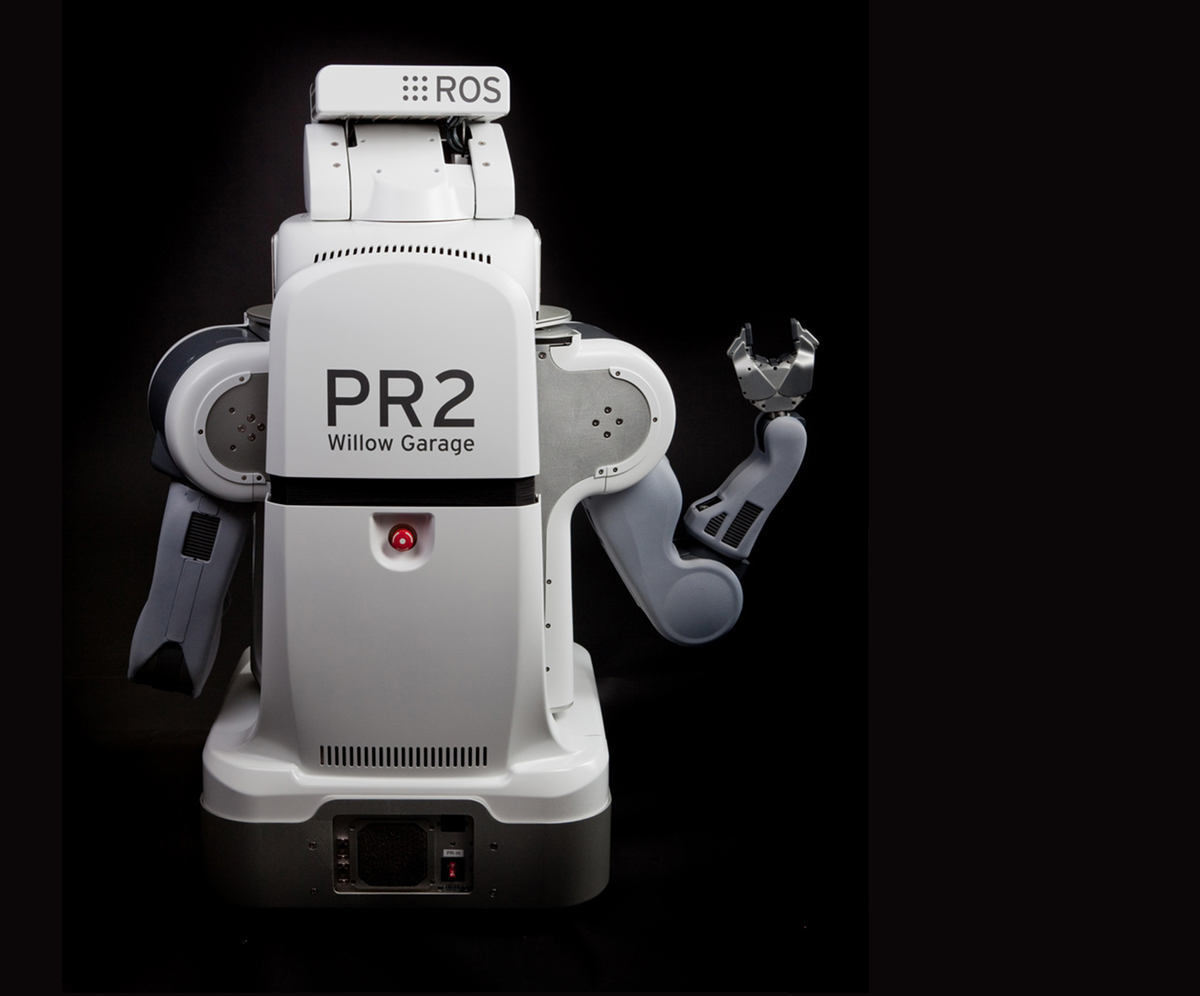
\includegraphics[scale=0.16]{Images/Chapter 1/PR2_Robot_Willow_Garage_6-1.jpeg}
    \caption{Willow Garage PR2 robot}
    \label{fig:PR2}
\end{figure}
\newpage
\section{Meta-Operating System}
ROS is an open source, meta operating framework for robots, hence it is nothing else than a middleware. \\
A middleware can be defined as a piece of software that gives an extra level of abstraction to the developer through a layer between the operating system and the applications.
It basically sits in the middle of software components and facilitates their interaction. \\
Its purpose is to provide an abstraction model for functions and at the same time provides the low-level implementation.
Every middleware must provide:
\begin{itemize}
    \item Portability: common programming model regardless the programming language and system architecture
    \item Complexity management: low-level aspects are managed by libraries and drivers inside the middleware itslef
    \item Reliability: middleware allows robot developer to discard low level details
    \item abstraction from sensors/actuators hardware;
    \item communication protocol for data transport
\end{itemize}
 As a result, they play an essential role in the development of complex applications that rely on a number of hardware and software tools.\\
 While they are still under active development, they are not yet capable of providing a complete set of functions for general purpose robots.
 
\begin{figure}[H]
    \centering
    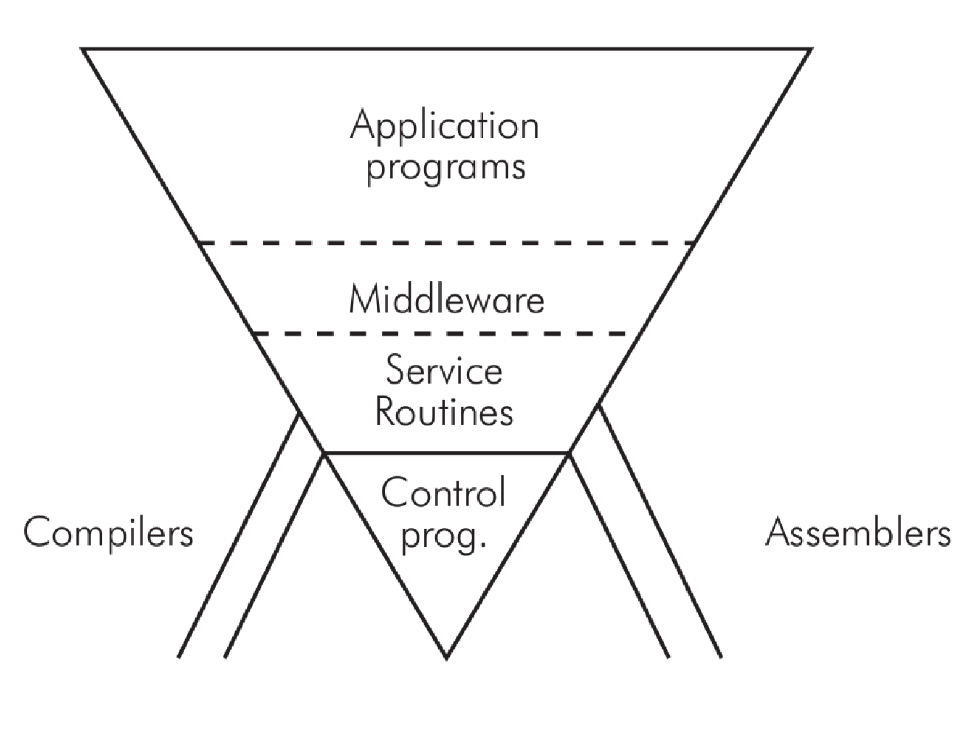
\includegraphics[scale=0.5]{Images/Chapter 1/middleware.png}
    \caption{Meta Operating System}
    \label{fig:metaoperating}
\end{figure}
 
 Several robotic middlewares have been proposed in the past years (OROCOS, ORCA, YARP, BRICS etc.) and eventually came ROS.
 
 \subsection{Phylosophy of ROS}
The following paragraphs describe some philosophical aspects of ROS:\\
\begin{itemize}
\item \textit{Peer to peer}: ROS systems consist of a small number of computer programs that are linked to one another and continuously exchange messages. These messages travel directly from one program to another. Although this makes the system more complex, the result is a system that balances better as the number of data increases.\\
\item \textit{Distributed}: Programs can be run on multiple computers and comunicate over the network.
\item \textit{Multilingual}: ROS chose a multilingual approach. ROS software modules can be written in any language for which a client library has been written. At the time of writing, client libraries exist for C++, Python, LISP, Java, JavaScript, MATLAB and others.\\
\item \textit{Thin}: the ROS conventions encourage contributors to create standalone libraries and then wrap those libraries, so that they can send and receive messages to and from other ROS modules. This extra layer is proposed to allow the reuse of software outside of ROS for other applications, and it greatly simplifies the creation of automated tests using standard continuous integration tools.\\
\item \textit{Free and open source}: the core of ROS is released under the permissive BSD license, which allows both commercial and non-commercial use. ROS foresees data exchange between modules using inter-process communication (IPC), which means that systems built using ROS can have fine-grained licensing of their various components.\\
\end{itemize}

\section{ROS Architecture}
ROS is based on a graph architecture where processing takes place in nodes, which communicate with each other by exchanging messages asynchronously through the use of topics to which they can subscribe to and/or on which they can publish, and synchronously with the calling of services, similar to RPCs.  Structurally, ROS is developed on 3 conceptual levels, File-system Level, Computational Level and Community Level, of which we are going to examine the constituent elements and their role in the architecture.
\subsection{File-system Level}
The Filesystem Level includes all resources used in ROS, in particular
\begin{itemize}
    \item Packages
    \item Metapackages
    \item Manifest
    \item Message types
    \item Service types
\end{itemize}
\begin{figure}
    \centering
    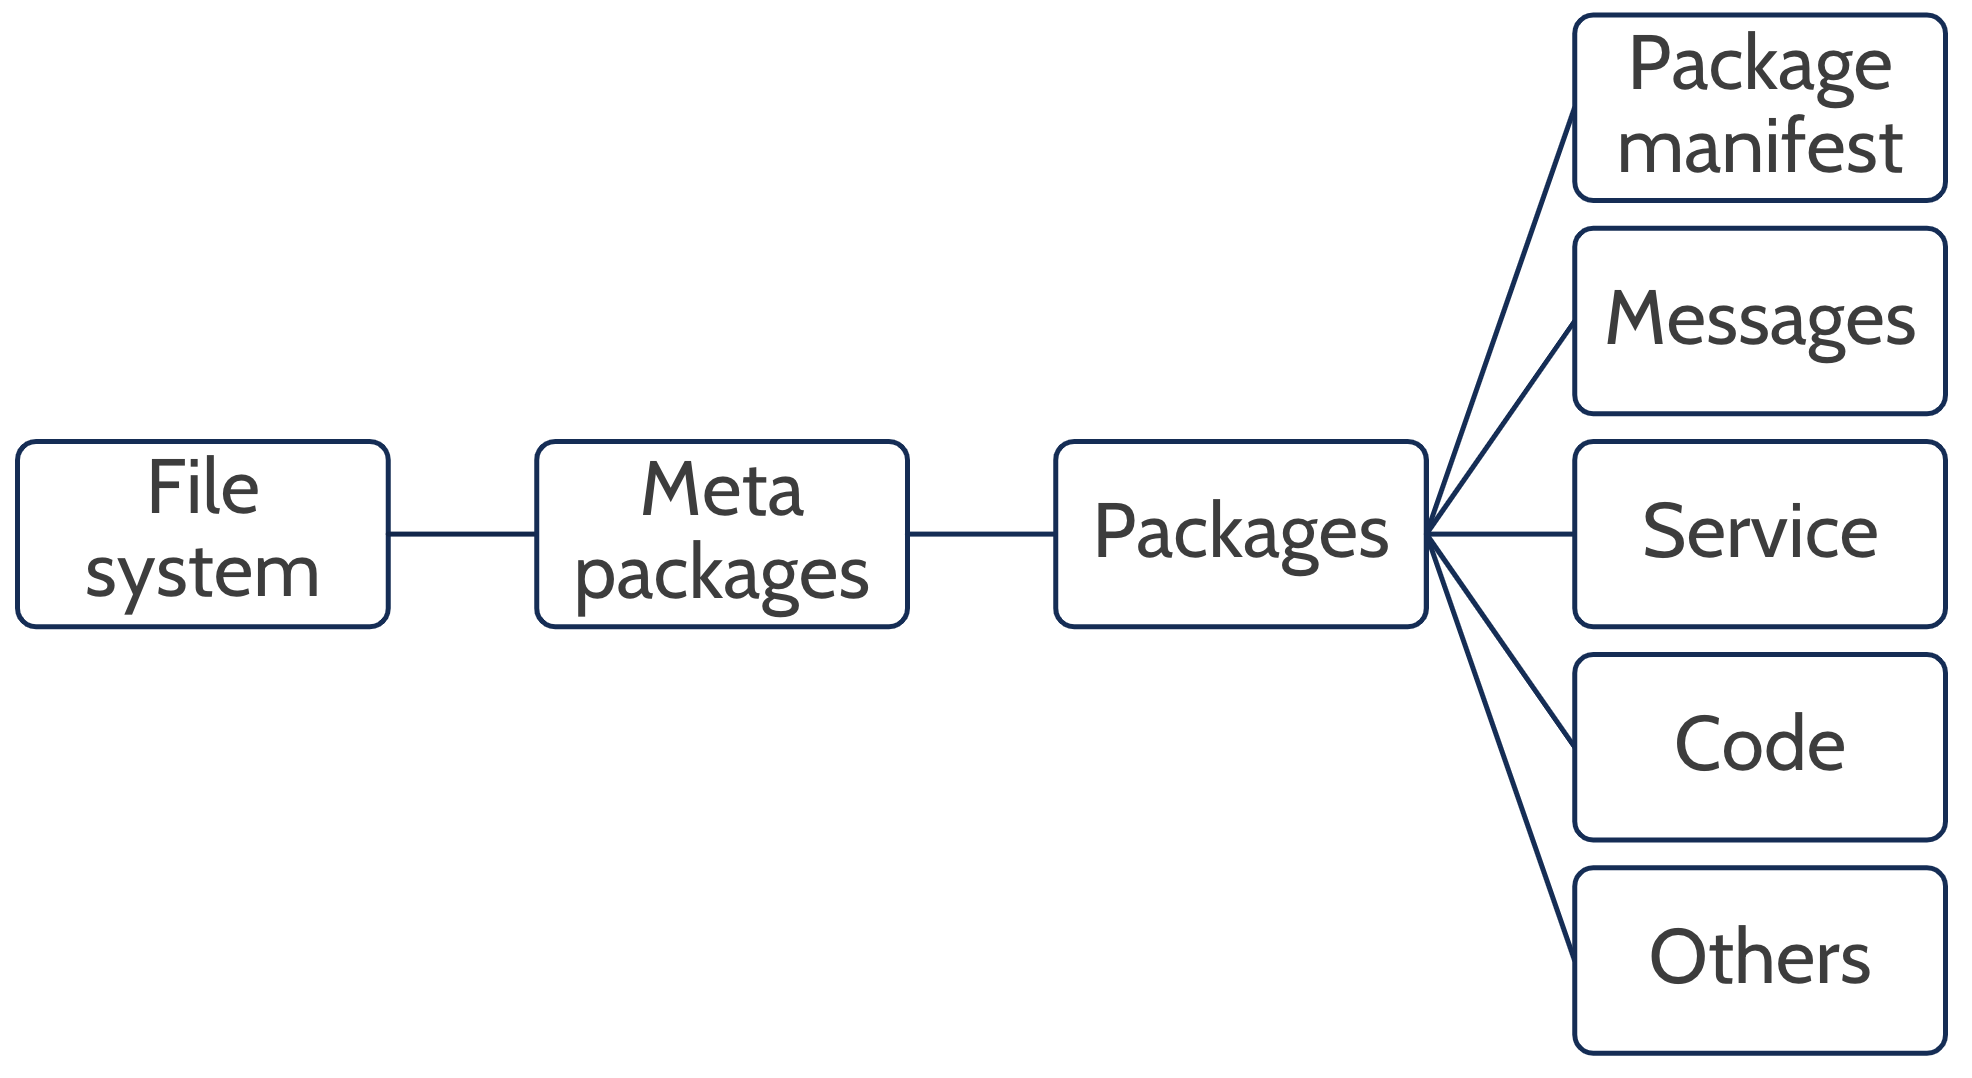
\includegraphics[scale=0.5]{Images/Chapter 1/Filesystem.png}
    \caption{File System level representation}
    \label{fig:Filesystem}
\end{figure}
\textbf{Packages}\\
Packages are the main structure for organising ROS  \citet{rospackages}. The processes, libraries, configuration files, datasets, and all the files used by the system at runtime are stored in these files. They are the structure that can be found within a ROS-based system. At the filesystem level, the package is represented by a directory. The structure within it includes some subfolders to manage the elements
In order to facilitate its development, in particular:
\begin{itemize}
    \item \textit{include/packagename}: C++ include headers (make sure to export in the CMakeLists.txt)
    \item \textit{msg}:Folder containing Message (msg) types
    \item \textit{src/packagename}: Source files, especially Python source that are exported to other packages.
    \item \textit{srv/}: Folder containing Service (srv) types
    \item \textit{scripts}: executable scripts
    \item \textit{CMakeLists.txt}: CMake build file
    \item \textit{package.xml}:XML file containing package structure 
    \item \textit{CHANGELOG.rst}: Many packages will define a changelog which can be automatically injected into binary packaging and into the wiki page for the package
\end{itemize}\\

\textbf{Metapackages}\\
Metapackages are specialised structures whose only task is to represent a group of packages that have common characteristics with each other. The metapackages that are created in the context of older versions of ROS and later updated may also result from the conversion of older stacks that perform similar functions in the context of older versions of ROS \citet{rosmetapackages}.\\
\newline
\textbf{Manifest}\\
A package manifest consists of an XML file named package.xml that must be included in the root folder of any catkin-compliant package. It contains information about the package, including its name, version number, authors, maintainers, and dependencies on other catkin packages. There is a strong similarity between this concept and the manifest.xml file used in the legacy rosbuild build system. System package dependencies are declared in package.xml \citet{rosmanifest}.\\
\newpage
There are a minimal set of tags that need to be nested within the <package> tag to make the package manifest complete.
\begin{itemize}
    \item \textit{<name>}: The name of the package
    \item \textit{<version>}: The version number of the package;
    \item \textit{<description>}: A description of the package contents;
    \item \textit{<maintainer>}: The name of the person(s) that is/are maintaining the package;
    \item \textit{<license}: The software license under which the code is released.
\end{itemize}
\textbf{Message types}\\
Message types define the structure of messages sent by ROS \citet{rosmsg}. Each file, with extension .msg, represents a different type of message. Within the file each line represents a message field. Each line, in turn, contains two columns: the first one for the data type of the field
(Int32/int (C++/Phyton), bool, string, time, etc.), the second for the name. It is possible to assign values to the fields within these le, in this case we speak of constants. Example of msg file (C++):

\textbf{Service types}\\
Service type are files that define the structure of request/response for ROS services \citet{rossrv}.
These are directly built upon the msg format to enable communication between nodes. They are stored in dedicated .srv files in the srv/ subdirectory of a package.
Example of srv file (C++):
\begin{lstlisting}[language=C++]
 bool add(beginner_tutorials::AddTwoInts::Request  &req,
             beginner_tutorials::AddTwoInts::Response &res)
    {
      res.sum = req.a + req.b;
      ROS_INFO("request: x=%ld, y=%ld", (long int)req.a, (long int)req.b);
      ROS_INFO("sending back response: [%ld]", (long int)res.sum);
     return true;
   }
\end{lstlisting}

\newpage

\subsection{ROS Computational Graph Level}
The Computation Graph is the peer-to-peer network of ROS processes that are processing data together. The basic Computation Graph concepts of ROS are nodes, Master, Parameter Server, messages, services, topics, and bags, all of which provide data to the Graph in different ways \citet{rosconcepts}.\\
\begin{figure}[H]
    \centering
    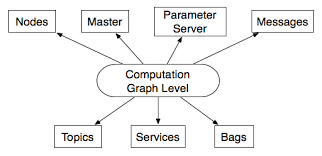
\includegraphics{Images/Chapter 1/computationgraph.png}
    \caption{Computation Graph}
    \label{fig:computationgraph}
\end{figure}
\textbf{Nodes}\\
A node is a process that performs computation. Nodes are combined together into a graph and communicate with one another using streaming topics, RPC services, and the Parameter Server \citet{rosnodes}. Following the concept of modularity of the system, each node will be related to only one specific functionality.\\ ROS in fact
discourages the creation of 'omnipotent' nodes that perform many functions in order to make the system more maintainable, reusable and clear.\\
The use of nodes in ROS provides several benefits to the overall system. There is additional fault tolerance as crashes are isolated to individual nodes. Code complexity is reduced in comparison to monolithic systems.\\
\newpage
\textbf{Topics}\\
Topics are buses identified by a proper and unique name that allow messages to be exchanged between nodes. They implement a mechanism
of publishing and subscribing: nodes can be publishers and/or subscribers if they are set up to send or receive messages. The division between
data producer and data user is clear and separated by anonymity policies
between the nodes. Each topic may have a maximum number of messages to be kept
in the queue in case they accumulate, those in excess are not added to the queue and lost \citet{rostopics}.\\
\newline
\textbf{Services}\\
Services are a two-way communication tool between nodes. It is a mechanism that extends that of messages with the possibility
not only to send commands to a specific node but also to remain in
listening and receiving a structured response from it. Each service is
first described in an .srv file where the parameters and type of service are indicated in addition to the name of the service.
of the service, as well as the parameters and the type of return data (see Service type).
Within the server node, the service is represented by a function
which takes as input two pointers to objects of the server class: one
one will include the function parameters (Request), the other will collect the return value.
will collect the return value \citet{rosservice}\\
\newline
\textbf{Messages}\\
The nodes in the graph communicate by exchanging messages. These
may be simple and of a primitive type (integer 
oat, string, char, etc.)
or arrays or even more complex, with structures similar to those seen in
C.\\
\newline
\textbf{Bags}\\
Bags represent the system by which ROS saves logs and keeps track of
all messages exchanged within a topic. The rosbag tool, once
associated with a topic, saves each message exchanged within a related file with the extension .bag. It is
very useful for storing data from the
sensors as it allows the developer to create a sort of "black box" of the robot.
black box" of the robot. ROS also provides a playback tool that allows the
visualise and playback the collected data via a graphical interface.\\
\newpage
\textbf{Master}\\
The master in ROS first takes care of registering new nodes within the
network, then managing the connection between the nodes in the graph, routing
messages and allowing access by one node to the services of another.
It is the heart of the software and can only be active one master at a time. It can be started via the roscore command or launched automatically
at the start of a node through the correct implementation of the file.
\begin{figure}[H]
    \centering
    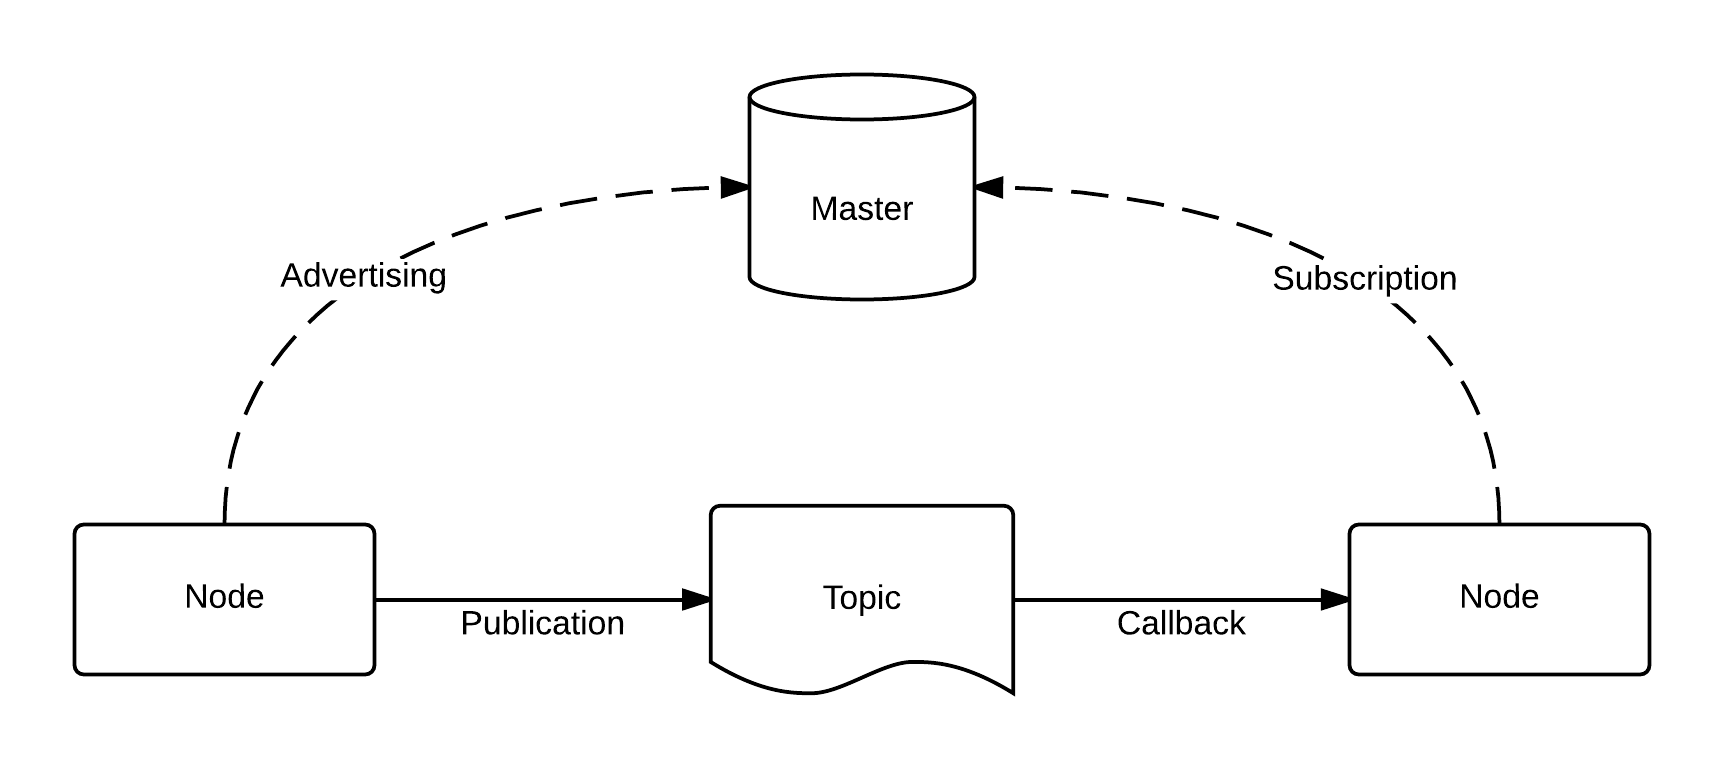
\includegraphics{Images/Chapter 1/ROS-master-node-topic.png}
    \caption{Visualization of Master-Node-Topic relationship}
    \label{fig:master-node-topic}
\end{figure}
\\
\newline
\textbf{Parameter server}\\
The parameter server is basically a component of the master, allowing certain configurations accessible via the network API to be shared publicly with all nodes. Although not an extremely high-performing it is nevertheless useful for the testing phase of the software. Parameters are named using the normal ROS naming convention. This means that ROS parameters have a hierarchy that matches the namespaces used for topics and nodes, \citet{rosparmserv}.

\chapter{Robot}
\label{robot}
\section{Introduction}
In the field of robotics, platforms are of increasing importance. A platform is divided into a software platform and a hardware platform. There are a variety of features that make up robot software platforms, including low-level device control, SLAM (Simultaneous Localization and Mapping), navigation, manipulation, recognition of objects or people, sensing and package management, debugging and development tools, which are mostly used in the industrial sector where robot software platforms are currently primarily employed. Robot hardware platforms not only study platforms such as mobile robots, drones, and humanoids, but also commercial products. Hence, robot researchers from around the world are collaborating to discover a platform that is intuitive and open source. The most popular robot software platform is ROS, that means Robot Operating System. ROS, the Robot Operating System, is an open source framework to manage robots’ operations, tasks, motions, and other things. ROS is intended to serve as a software platform for those who build and use robots daily, but at the same time for people who are starting to use robots no long ago. This common platform allows newcomers to be increasingly inclined to read more and more and it is very easy to use. The design of the ROS platform allows the use of code and information shared by other programmers, which means you do not have to write all code in order to move the robots.
\newpage
\section{History of ROS}
“In May 2007, ROS was started by borrowing the early opensource robotic software frameworks including switchyard, which is developed by Dr. Morgan Quigley by the Stanford Artificial Intelligence Laboratory in support of the Stanford AI Robot STAIR (Stanford AI Robot) project.
Dr. Morgan Quigley is one of the founders and software development manager of Open Robotics (formerly the Open Source Robotics Foundation, OSRF), which is responsible for the development and management of ROS.
Switchyard is a program created for the development of artificial intelligence robots used in the AI lab’s projects at the time and it is the predecessor of ROS.
In addition, Dr. Brian Gerkey, the developer of the Player/Stage Project and 2D Stage simulator, later influence the growth of 3D simulator Gazebo, which was developed since 2000 and has had a major impact on ROS’s networking program. He is the co-founder of Open Robotics.
In November 2007, U.S. robot company Willow Garage succeeded the development of ROS. Willow Garage is a well-known company in the field of personal robots and service robots.” \cite{Quigley15}\\
Robots are computer-controlled electromechanical devices.
First dedicated robot programming languages arose in the 1970's.
There were robot-centric data types and some robot function libraries. They did not allow neither hardware abstractio, nor multi-robot interaction nor integrated simulation. There did not exist code reuse or standardization.
The efforts to build robot programming system continued through 80's, 90's and especially in the 2000's were there was a high push to standardize robot components, their interfaces and basic functions.\\
Hence, ROS as it is known today was initially developed in 2007 at the Standford Artificial Intelligence Laboratory. Since 2013 it is managed by OSRF and nowadays it is used by many robots, universities and companies, becoming the de facto standard for robot programming.
\begin{figure}[H]
    \centering
    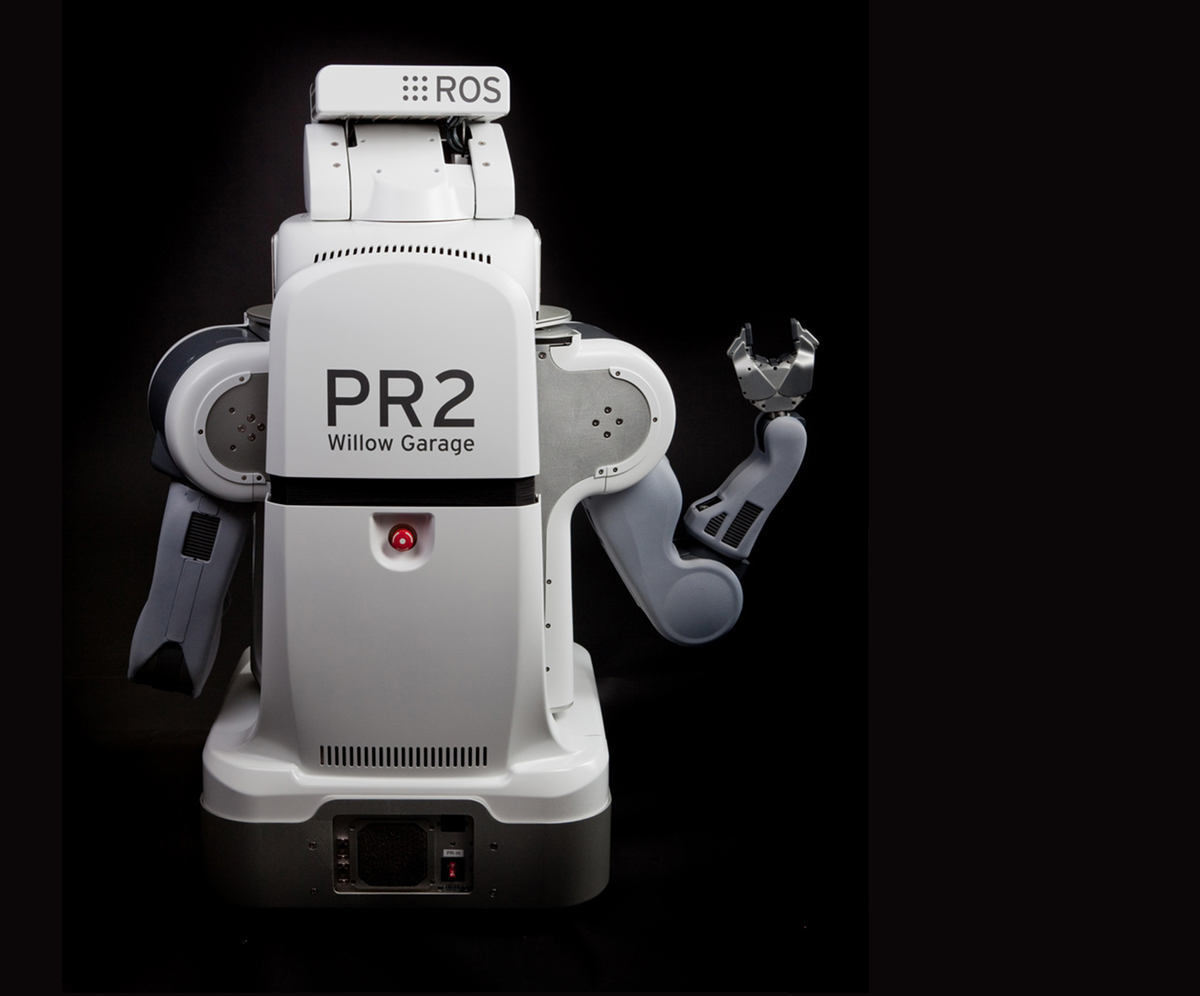
\includegraphics[scale=0.16]{Images/Chapter 1/PR2_Robot_Willow_Garage_6-1.jpeg}
    \caption{Willow Garage PR2 robot}
    \label{fig:PR2}
\end{figure}
\newpage
\section{Meta-Operating System}
ROS is an open source, meta operating framework for robots, hence it is nothing else than a middleware. \\
A middleware can be defined as a piece of software that gives an extra level of abstraction to the developer through a layer between the operating system and the applications.
It basically sits in the middle of software components and facilitates their interaction. \\
Its purpose is to provide an abstraction model for functions and at the same time provides the low-level implementation.
Every middleware must provide:
\begin{itemize}
    \item Portability: common programming model regardless the programming language and system architecture
    \item Complexity management: low-level aspects are managed by libraries and drivers inside the middleware itslef
    \item Reliability: middleware allows robot developer to discard low level details
    \item abstraction from sensors/actuators hardware;
    \item communication protocol for data transport
\end{itemize}
 As a result, they play an essential role in the development of complex applications that rely on a number of hardware and software tools.\\
 While they are still under active development, they are not yet capable of providing a complete set of functions for general purpose robots.
 
\begin{figure}[H]
    \centering
    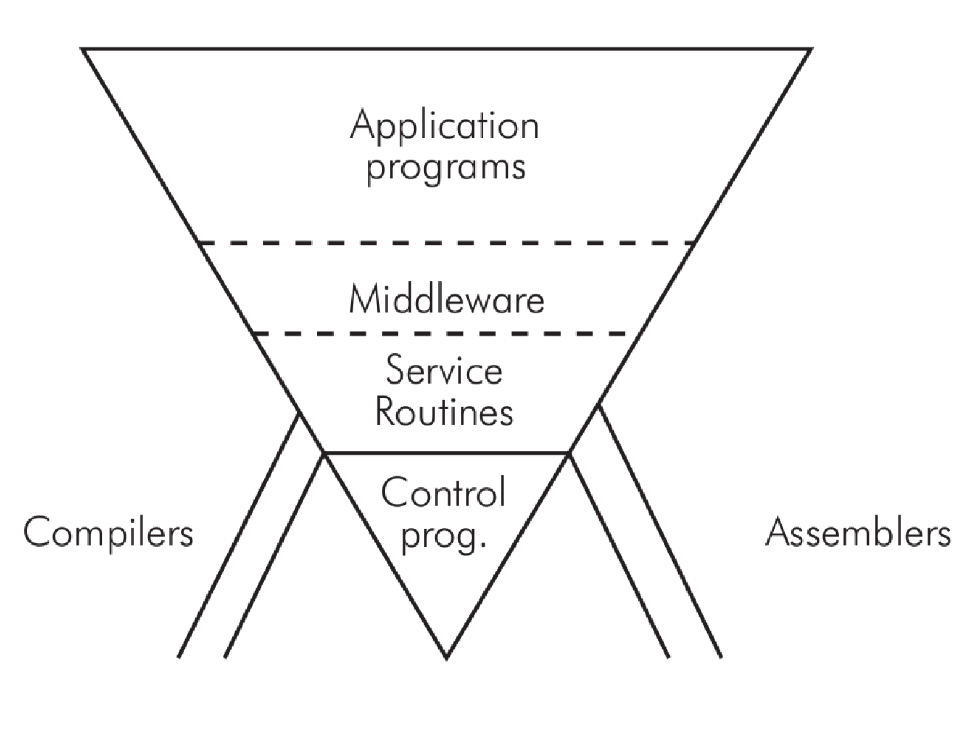
\includegraphics[scale=0.5]{Images/Chapter 1/middleware.png}
    \caption{Meta Operating System}
    \label{fig:metaoperating}
\end{figure}
 
 Several robotic middlewares have been proposed in the past years (OROCOS, ORCA, YARP, BRICS etc.) and eventually came ROS.
 
 \subsection{Phylosophy of ROS}
The following paragraphs describe some philosophical aspects of ROS:\\
\begin{itemize}
\item \textit{Peer to peer}: ROS systems consist of a small number of computer programs that are linked to one another and continuously exchange messages. These messages travel directly from one program to another. Although this makes the system more complex, the result is a system that balances better as the number of data increases.\\
\item \textit{Distributed}: Programs can be run on multiple computers and comunicate over the network.
\item \textit{Multilingual}: ROS chose a multilingual approach. ROS software modules can be written in any language for which a client library has been written. At the time of writing, client libraries exist for C++, Python, LISP, Java, JavaScript, MATLAB and others.\\
\item \textit{Thin}: the ROS conventions encourage contributors to create standalone libraries and then wrap those libraries, so that they can send and receive messages to and from other ROS modules. This extra layer is proposed to allow the reuse of software outside of ROS for other applications, and it greatly simplifies the creation of automated tests using standard continuous integration tools.\\
\item \textit{Free and open source}: the core of ROS is released under the permissive BSD license, which allows both commercial and non-commercial use. ROS foresees data exchange between modules using inter-process communication (IPC), which means that systems built using ROS can have fine-grained licensing of their various components.\\
\end{itemize}

\section{ROS Architecture}
ROS is based on a graph architecture where processing takes place in nodes, which communicate with each other by exchanging messages asynchronously through the use of topics to which they can subscribe to and/or on which they can publish, and synchronously with the calling of services, similar to RPCs.  Structurally, ROS is developed on 3 conceptual levels, File-system Level, Computational Level and Community Level, of which we are going to examine the constituent elements and their role in the architecture.
\subsection{File-system Level}
The Filesystem Level includes all resources used in ROS, in particular
\begin{itemize}
    \item Packages
    \item Metapackages
    \item Manifest
    \item Message types
    \item Service types
\end{itemize}
\begin{figure}
    \centering
    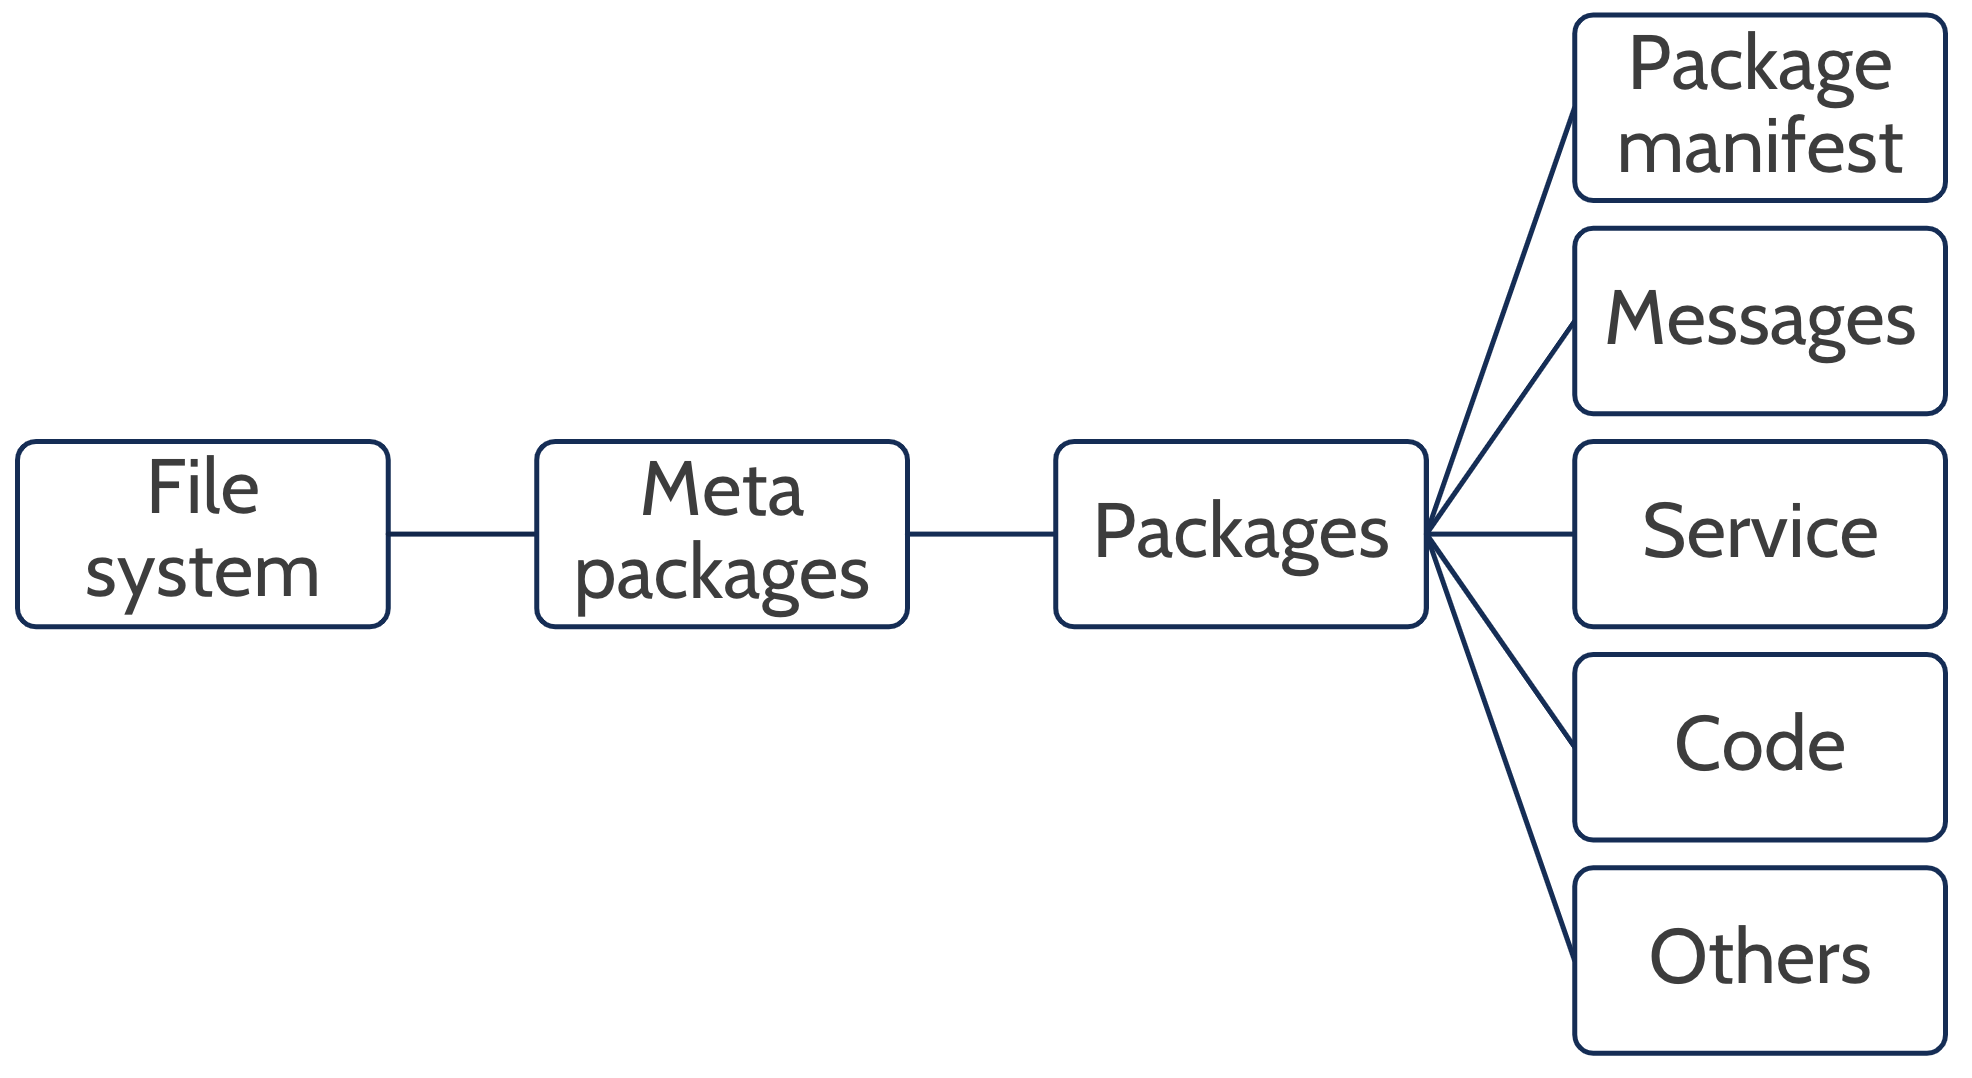
\includegraphics[scale=0.5]{Images/Chapter 1/Filesystem.png}
    \caption{File System level representation}
    \label{fig:Filesystem}
\end{figure}
\textbf{Packages}\\
Packages are the main structure for organising ROS  \citet{rospackages}. The processes, libraries, configuration files, datasets, and all the files used by the system at runtime are stored in these files. They are the structure that can be found within a ROS-based system. At the filesystem level, the package is represented by a directory. The structure within it includes some subfolders to manage the elements
In order to facilitate its development, in particular:
\begin{itemize}
    \item \textit{include/packagename}: C++ include headers (make sure to export in the CMakeLists.txt)
    \item \textit{msg}:Folder containing Message (msg) types
    \item \textit{src/packagename}: Source files, especially Python source that are exported to other packages.
    \item \textit{srv/}: Folder containing Service (srv) types
    \item \textit{scripts}: executable scripts
    \item \textit{CMakeLists.txt}: CMake build file
    \item \textit{package.xml}:XML file containing package structure 
    \item \textit{CHANGELOG.rst}: Many packages will define a changelog which can be automatically injected into binary packaging and into the wiki page for the package
\end{itemize}\\

\textbf{Metapackages}\\
Metapackages are specialised structures whose only task is to represent a group of packages that have common characteristics with each other. The metapackages that are created in the context of older versions of ROS and later updated may also result from the conversion of older stacks that perform similar functions in the context of older versions of ROS \citet{rosmetapackages}.\\
\newline
\textbf{Manifest}\\
A package manifest consists of an XML file named package.xml that must be included in the root folder of any catkin-compliant package. It contains information about the package, including its name, version number, authors, maintainers, and dependencies on other catkin packages. There is a strong similarity between this concept and the manifest.xml file used in the legacy rosbuild build system. System package dependencies are declared in package.xml \citet{rosmanifest}.\\
\newpage
There are a minimal set of tags that need to be nested within the <package> tag to make the package manifest complete.
\begin{itemize}
    \item \textit{<name>}: The name of the package
    \item \textit{<version>}: The version number of the package;
    \item \textit{<description>}: A description of the package contents;
    \item \textit{<maintainer>}: The name of the person(s) that is/are maintaining the package;
    \item \textit{<license}: The software license under which the code is released.
\end{itemize}
\textbf{Message types}\\
Message types define the structure of messages sent by ROS \citet{rosmsg}. Each file, with extension .msg, represents a different type of message. Within the file each line represents a message field. Each line, in turn, contains two columns: the first one for the data type of the field
(Int32/int (C++/Phyton), bool, string, time, etc.), the second for the name. It is possible to assign values to the fields within these le, in this case we speak of constants. Example of msg file (C++):

\textbf{Service types}\\
Service type are files that define the structure of request/response for ROS services \citet{rossrv}.
These are directly built upon the msg format to enable communication between nodes. They are stored in dedicated .srv files in the srv/ subdirectory of a package.
Example of srv file (C++):
\begin{lstlisting}[language=C++]
 bool add(beginner_tutorials::AddTwoInts::Request  &req,
             beginner_tutorials::AddTwoInts::Response &res)
    {
      res.sum = req.a + req.b;
      ROS_INFO("request: x=%ld, y=%ld", (long int)req.a, (long int)req.b);
      ROS_INFO("sending back response: [%ld]", (long int)res.sum);
     return true;
   }
\end{lstlisting}

\newpage

\subsection{ROS Computational Graph Level}
The Computation Graph is the peer-to-peer network of ROS processes that are processing data together. The basic Computation Graph concepts of ROS are nodes, Master, Parameter Server, messages, services, topics, and bags, all of which provide data to the Graph in different ways \citet{rosconcepts}.\\
\begin{figure}[H]
    \centering
    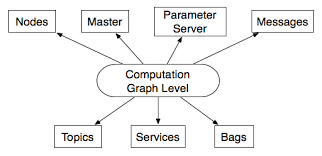
\includegraphics{Images/Chapter 1/computationgraph.png}
    \caption{Computation Graph}
    \label{fig:computationgraph}
\end{figure}
\textbf{Nodes}\\
A node is a process that performs computation. Nodes are combined together into a graph and communicate with one another using streaming topics, RPC services, and the Parameter Server \citet{rosnodes}. Following the concept of modularity of the system, each node will be related to only one specific functionality.\\ ROS in fact
discourages the creation of 'omnipotent' nodes that perform many functions in order to make the system more maintainable, reusable and clear.\\
The use of nodes in ROS provides several benefits to the overall system. There is additional fault tolerance as crashes are isolated to individual nodes. Code complexity is reduced in comparison to monolithic systems.\\
\newpage
\textbf{Topics}\\
Topics are buses identified by a proper and unique name that allow messages to be exchanged between nodes. They implement a mechanism
of publishing and subscribing: nodes can be publishers and/or subscribers if they are set up to send or receive messages. The division between
data producer and data user is clear and separated by anonymity policies
between the nodes. Each topic may have a maximum number of messages to be kept
in the queue in case they accumulate, those in excess are not added to the queue and lost \citet{rostopics}.\\
\newline
\textbf{Services}\\
Services are a two-way communication tool between nodes. It is a mechanism that extends that of messages with the possibility
not only to send commands to a specific node but also to remain in
listening and receiving a structured response from it. Each service is
first described in an .srv file where the parameters and type of service are indicated in addition to the name of the service.
of the service, as well as the parameters and the type of return data (see Service type).
Within the server node, the service is represented by a function
which takes as input two pointers to objects of the server class: one
one will include the function parameters (Request), the other will collect the return value.
will collect the return value \citet{rosservice}\\
\newline
\textbf{Messages}\\
The nodes in the graph communicate by exchanging messages. These
may be simple and of a primitive type (integer 
oat, string, char, etc.)
or arrays or even more complex, with structures similar to those seen in
C.\\
\newline
\textbf{Bags}\\
Bags represent the system by which ROS saves logs and keeps track of
all messages exchanged within a topic. The rosbag tool, once
associated with a topic, saves each message exchanged within a related file with the extension .bag. It is
very useful for storing data from the
sensors as it allows the developer to create a sort of "black box" of the robot.
black box" of the robot. ROS also provides a playback tool that allows the
visualise and playback the collected data via a graphical interface.\\
\newpage
\textbf{Master}\\
The master in ROS first takes care of registering new nodes within the
network, then managing the connection between the nodes in the graph, routing
messages and allowing access by one node to the services of another.
It is the heart of the software and can only be active one master at a time. It can be started via the roscore command or launched automatically
at the start of a node through the correct implementation of the file.
\begin{figure}[H]
    \centering
    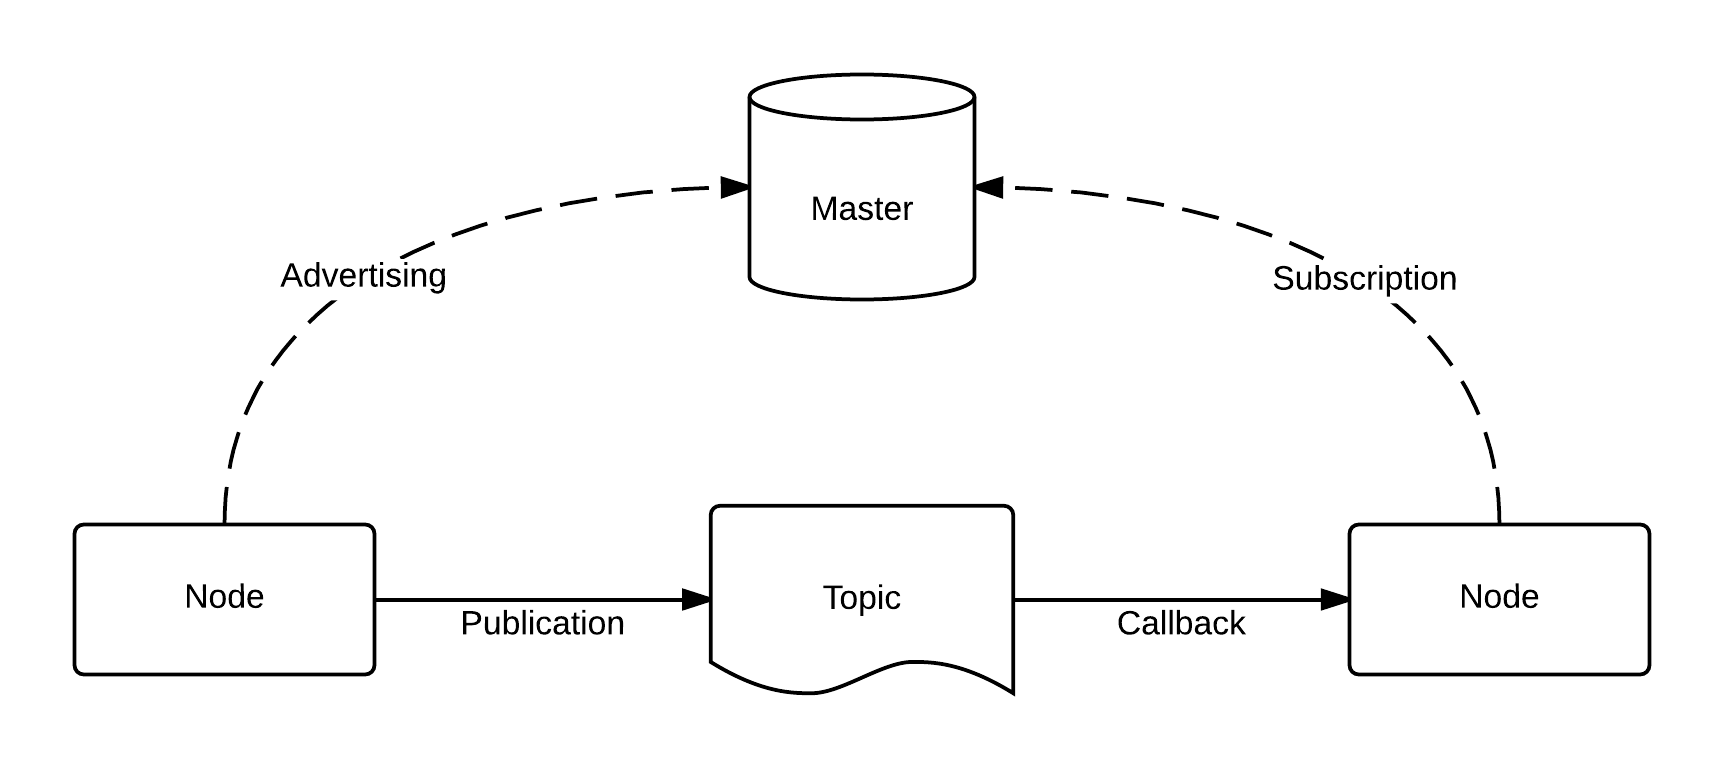
\includegraphics{Images/Chapter 1/ROS-master-node-topic.png}
    \caption{Visualization of Master-Node-Topic relationship}
    \label{fig:master-node-topic}
\end{figure}
\\
\newline
\textbf{Parameter server}\\
The parameter server is basically a component of the master, allowing certain configurations accessible via the network API to be shared publicly with all nodes. Although not an extremely high-performing it is nevertheless useful for the testing phase of the software. Parameters are named using the normal ROS naming convention. This means that ROS parameters have a hierarchy that matches the namespaces used for topics and nodes, \citet{rosparmserv}.


\chapter{Conclusions and future developments}
\label{ch:conclusions}%
A final chapter containing the main conclusions of your research/study
and possible future developments of your work have to be inserted in this chapter.

%-------------------------------------------------------------------------
%	BIBLIOGRAPHY
%-------------------------------------------------------------------------

\addtocontents{toc}{\vspace{2em}} % Add a gap in the Contents, for aesthetics
\bibliography{Thesis_bibliography} % The references information are stored in the file named "Thesis_bibliography.bib"

%-------------------------------------------------------------------------
%	APPENDICES
%-------------------------------------------------------------------------

\cleardoublepage
\addtocontents{toc}{\vspace{2em}} % Add a gap in the Contents, for aesthetics
\appendix
\chapter{Appendix A}
If you need to include an appendix to support the research in your thesis, you can place it at the end of the manuscript.
An appendix contains supplementary material (figures, tables, data, codes, mathematical proofs, surveys, \dots)
which supplement the main results contained in the previous chapters.

\chapter{Appendix B}
It may be necessary to include another appendix to better organize the presentation of supplementary material.


% LIST OF FIGURES
\listoffigures

% LIST OF TABLES
\listoftables

% LIST OF SYMBOLS
% Write out the List of Symbols in this page
\chapter*{List of Symbols} % You have to include a chapter for your list of symbols (
\begin{table}[H]
    \centering
    \begin{tabular}{lll}
        \textbf{Variable} & \textbf{Description} & \textbf{SI unit} \\\hline\\[-9px]
        $\bm{u}$ & solid displacement & m \\[2px]
        $\bm{u}_f$ & fluid displacement & m \\[2px]
    \end{tabular}
\end{table}

% ACKNOWLEDGEMENTS
\chapter*{Acknowledgements}
Here you might want to acknowledge someone.

\cleardoublepage

\end{document}
